\section{Desarrollo}

\subsection{Calibración}

El primer paso para comenzar el algoritmo de fotometría estéreo es realizar
la calibración del sistema. Para cada objeto, contamos con 12 imágenes,
cada una con una fuente de iluminación distinta; es decir, la dirección o
ángulo de incidencia de la luz es diferente. El objetivo del paso de calibración
es calcular la dirección de cada fuente de iluminación.

A este efecto, contamos con un conjunto de imágenes de referencia iluminadas
con los mismos ángulos que el objeto a analizar, pero con la ventaja de que se
trata de una esfera. Al tener una forma conocida y simple, podemos conocer con
exactitud la profundidad y posición espacial de cada punto del objeto,
sabiendo el centro y el radio de la misma siguiendo la siguiente ecuación:

\begin{center}
$(x - x_0)^2 + (y - y_0)^2 + (z - z_0)^2 = r^2$
\end{center}

Si definimos $z_0 = 0$ (es decir, si asumimos que la esfera está centrada
respecto del eje z), podemos calcular el vector normal a cada punto de la esfera:

\begin{center}
$n = (x - x_0, y - y0, z)$
\end{center}

Para los propósitos de este trabajo, vamos a asumir que los objetos tienen
superficies lambertiana, por lo que la intensidad del brillo de un punto
particular solo depende de la orientación de la superficie respecto de la
fuente de iluminación. Es decir, el punto de mayor intensidad lumínica
será el más cercano a la fuente de iluminación, por lo que la normal
de dicho punto apuntará en dirección a la fuente. El vector opuesto a esta
normal tiene la dirección de la fuente.

Si se ejecuta este procedimiento para las 12 imágenes de la esfera, entonces
el resultado será conocer la dirección de las 12 fuentes de iluminación. Esto,
combinado con las imágenes correspondientes de la figura a procesar,
nos permitirá calcular la normal para cada punto de la figura.

\subsection{Reconstrucción del modelo 3D de los objetos digitalizados}

Una vez completada la calibración, ya se cuenta con las direcciones de
iluminación de cada caso, las cuales junto con la secuencia de imágenes de un
objeto nos proporcionarán la información necesaria para poder calcular todos
los puntos $(x,y,z)$ del modelo digitalizado y las normales de cada uno.

Para las siguientes secciones, se aplicó una máscara del objeto la cual está compuesta por una parte blanca en donde se encuentra el objeto en las imagenes originales y todo el resto de negro. De esta forma, se puede ubicar fácilmente dónde está el objeto a reconstruir y por lo tanto no generar vectores basura al rededor del mismo. Al mismo tiempo, la máscara permite recortar en un rectángulo más pequeño al objeto para así no tener que recorrer toda la imagen completa. Esto funciona ya que es buscar el pixel blanco que se encuentre más cerca del borde en cada uno de los lados. El algoritmo funciona y a mayor velocidad a causa de este recorte ya que omite gran cantidad de pixeles que se puede asegurar que no aportan información.

\subsubsection{Contrucción del campo normal}

En este paso se desea obtener la normal de cada punto del objeto. Para ello
se recurre a la ecuación 5 del enunciado de este trabajo práctico, que
vincula una matriz formada por 3 direcciones de fuentes de iluminación con el
vector $m$ y las intensidades del píxel en cada imágen. Esta matriz tiene 3
direcciones porque es la cantidad mínima de imágenes cuya fuente de
iluminación difiera entre sí necesaria para inferir la orientación de la
superficie.

La matriz de direcciones contiene la dirección de cada fuente de iluminación
dispuesta como fila. Una vez resuelto el sistema de ecuaciones se podrá
conocer $m$ y asi mediante la siguiente ecuacion $||m|| = |I_0\rho| ||n||$,
conocer el valor absoluto de $I_0\rho$. Esto permite conocer $n$ ya que tiene
la misma dirección que $m$ con la diferencia de que $n$ está normalizado
por ser la norma. Por lo que nos queda que $n = \frac{m}{||m||}$.

\subsubsection{Estimacion de la profundidad}

El siguiente paso es calcular la profundidad de cada pixel de la imagen. Para ello se recurre a las ecuaciones 11 y 12 del enunciado en donde se vincula a la normal de cada pixel con su profundidad. Estas ecuaciones nos permiten formar un sistema de ecuaciones como el de la ecuación 13.

Es necesario notar que $M$, la matriz de este sistema, es una matriz esparsa. La manera en la que la está dispuesta la información es la siguiente:

$M$ tiene dimensión $2n \times n$. Esto es porque necesitamos representar 2 ecuaciones por cada pixel, por lo que cada columna de $M$ referirá a $1$ pixel de la imagen y cada fila a una ecuación. Dado que cada pixel utiliza en las ecuaciones a los pixels de la derecha y de abajo, cada columna tendrá a lo sumo 4 elementos (dos por sus propias ecuaciones, una vez por el pixel de su izquierda y otra por el de arriba). Para el caso de los pixels de los bordes derechos e inferiores, solamente tendrán 2 elementos, que se dan por los pixeles que estan en la anteúltima columna y anteúltima fila de la imagen correspondientemente. El último pixel, el que se encuentra en la esquina inferior derecha, no tendrá ningún elemento en su respectiva columna.

Nuestra implementación consiste en considerar a esta matriz como un tipo especial de matriz (la esparsa), para la cual no se tiene un arreglo bidimensional como sería el caso habitual sino un vector de hashmap, donde cada elemento del vector representa una columna. Cada hashmap contendrá entonces 4 elementos o menos. Esto permite que al querer multiplicar una columna por otra (como ocurre en el caso de querer calcular $M^tM$) no sea necesario recorrer toda la columna sino únicamente los elementos distintos de 0. Esta optimización es crucial para el desarrollo del algoritmo a nivel temporal. Además, por cuestiones implementativas, se decidió utilizar un diccionario que mapea cada pixel a una columna, para así poder ubicar rápidamente en $z$ (una vez resuelto el sistema) el valor correspondiente a cada pixel.

Luego resta resolver el sistema de la ecuación 15. Para ello aplicamos la factorización de Cholesky, que también resulta optimizada debido a tratarse de una matriz esparsa, ya que para el cálculo de la matriz triangular inferior es necesario recorrer lo calculado en las iteraciones previas, y al utilizar la implementación de matriz esparsa definida anteriormente se logra recorrer la matriz solamente en los elementos distintos de 0.


\subsection{Experimentación}

En este trabajo se realizaron una serie de experimentaciones para poder responder preguntas planteadas en el enunciado. Se explica el detalle de las respuestas obtenidas en las siguientes subsecciones, pero a modo de introducción de esa parte indicamos que no se obtuvieron respuestas para todas las respuestas, pero las pruebas sirvieron para acercarse a una idea de las mismas.

\subsubsection{Análisis cuantitativo}

Con motivo de la construcción del campo normal se vio la necesidad de despejar el vector $m$ de la ecuación 5. El método conocido para esto es la \textit{Eliminación Gaussiana} (EG). Este método se aplica para resolver sistemas lineales de la forma: $Ax = b$. El método de \textit{Eliminación Gaussiana}, consiste en escalonar la matriz aumentada del sistema.

El problema que tiene este método es que no puede ser utilizado si en la diagonal de la matriz se encuentran ceros. Para evitar este problema se elige como elemento para hacer ceros (el cual recibe el nombre de elemento pivotal o simplemente pivote) como el elemento mayor en valor absoluto de entre todos los candidatos. A este procedimiento se le llama pivoteo parcial y aplicado a la \textit{Eliminación Gaussiana}, nos dá el llamado método de \textit{Eliminación Gaussiana con pivoteo}.

En este caso, se hace uso justamente de la \textit{Eliminación Gaussiana con pivoteo} donde se elige como elemento al mayor dentro de la columna. Esto garantiza que no hayan ceros en la diagonal, y al elegir al máximo se reducen lo más posible los errores numéricos.

Al momento de calcular las profundidades de los píxeles es necesario la utilización del método de \textit{Factorización de Cholesky} (CL). Cuando es aplicable, la descomposición de Cholesky es dos veces más eficiente que la descomposición LU. Una vez obtenida la factorización se puede fácilmente resolver el sistema de equaciónes pero no es posible obtener la factorización en cualquier caso.

El requisito para poder aplicar esta factorización es que la matriz sea simétrica definida positiva. En el caso de este trabajo práctico, la matriz en cuestión es producto de una matriz por su traspuesta, por lo que es sumétrica definida positiva ya que

\begin{center}
$x^tM^tMx = (Mx)^t(Mx) = ||Mx||^2 > 0$
\end{center}

Se realizó como prueba la comparación de tiempo y calidad de una imagen de tamaño normal contra la de una imagen de tamaño reducido 6 veces. El tiempo obtenido para la imagen chica fue de 0.146022 segundos, mientras que para la grande fue de 117.572 segundos. Dado que los algoritmos no son lineales, es una diferencia esperable. En cuanto a la calidad de la solución obtenida, se notó que para la imagen chica parecía dar profundidades de mejor calidad. Se muestra en las siguientes imágenes ambos resultados utilizando el gato como ejemplo:

\begin{center}
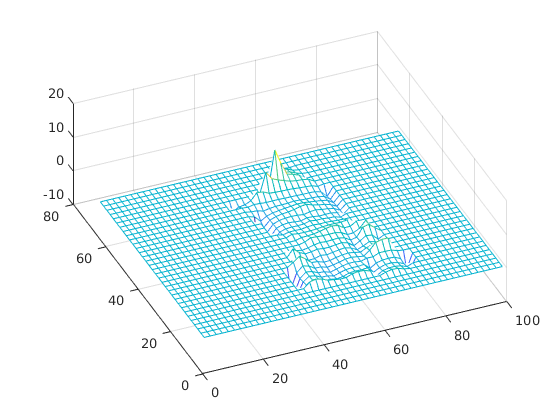
\includegraphics[width=.4\linewidth]{imagenes/gato_small_model_1511.png}
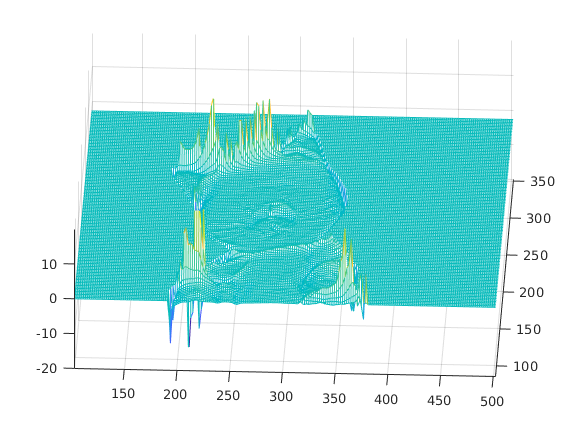
\includegraphics[width=.4\linewidth]{imagenes/gato_model_1511.png}
\end{center}


\subsubsection{Análisis cualitativo}

\paragraph{Luces por calibración VS Luces de la cátedra}
\

Luego de calibrar el sistema con las imágenes de referencia, decidimos comparar
las direcciones de luz obtenidas con aquellas provistas por la cátedra. Notamos
que nuestras direcciones no se coincidían perfectamente con las luces pre-computadas.

Consideramos que esto se debe a irregularidades en el color de la esfera. Si bien la misma
tiene una superficie lambertiana, el color de la misma no es uniforme, por lo que no
todos los puntos reflejan la luz de la misma forma. Un sector más oscuro de la esfera
puede reflejar menos la luz aunque la misma incida de forma directa. Por esto, nuestro proceso
de calibración podría confundir un punto particular de mayor intensidad con el punto de
incidencia directa de la luz.

En general, consideramos que nuestras estimaciones de las luces son suficientes.
Sin embargo, esto no siempre es cierto, ya que hay casos donde la diferencia
entre nuestras luces calibradas y la referencia de la cátedra difiere significativamente.

Si consideramos cada dirección de luz como vector, la norma de la diferencia
entre los vectores estimados y los de referencia varía entre 0,075 y 0,35.
Considerando que los vectores están normalizados, esta última diferencia es muy elevada.
Sin embargo, se trata de un caso extremo, siendo el promedio (0,14)
bastante menor, aunque no insignificante.

En particular, hallamos algunos casos en los cuales las luces calibradas coinciden casi
completamente, si bien la dirección real de la luz no era tan similar. Esto resulta en
combinaciones de luces que no producen resultados, ya que no satisfacen el
requerimiento de 3 luces distintas para la reconstrucción del objeto 3D.
En la siguiente sección se trata con mayor detalle.

\paragraph{Calibración y repercusiones}
\

El objetivo de la calibración es obtener suficiente información sobre cada punto
para determinar sus 3 componentes espaciales. Por esto, es necesario tener 3
fuentes de luz cuyas direcciones sean linealmente independientes.

Como se mencionó antes, existen casos donde las luces calibradas no resultaban
linealmente independientes (si bien las fuentes de iluminación no eran las mismas).
El resultado final es que no existe suficiente información sobre cada punto
para generar un campo normal, y por ende no se pueden estimar las profundidades.

En nuestro caso, las imágenes 3 y 5 (comenzando en 0) resultaron conflictivas,
ya que ambas tienen un mismo punto brillante que no corresponde con la dirección
de la luz. Por ende, nuestro proceso de calibración confunde ambas imágenes,
resultando en un sistema singular.

Por otro lado, si la calibración no es fiel, esto puede introducir ruido en
la construcción de los cuerpos, ya que la iluminación de cada punto no
se condice con el ángulo de incidencia de la luz establecido.

En las siguientes imágenes, se puede observar el ruido que introduce la calibración
imprecisa (izquierda) comparada con las direcciones correctas de las luces utilizadas
(derecha) para casos extremos de imprecisión:

\begin{center}
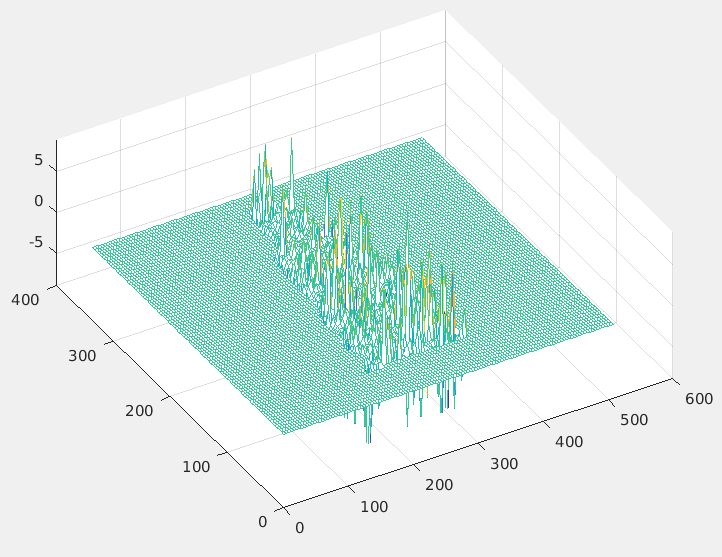
\includegraphics[width=.4\linewidth]{imagenes/calib-ruido.png}
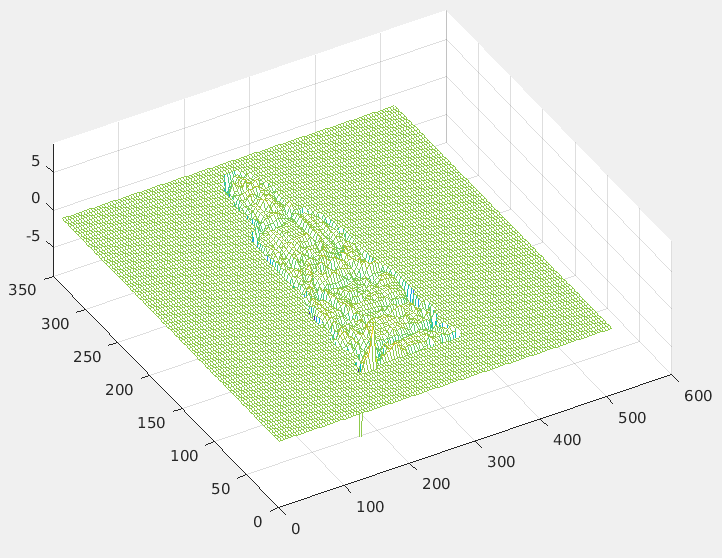
\includegraphics[width=.4\linewidth]{imagenes/luces-limpio.png}
\end{center}

\paragraph{Elección de las luces}
\

A lo largo del desarrollo, se observó que utilizando las mismas luces se obtenian diferentes calidades de modelos 3D para las distintas imágenes. Esto generó dudas de si el algoritmo para la reconstrucción del modelo estaba bien hecho ya que supusimos que la calidad debería ser igual para todas si se usaba siempre las mismas luces, pero al ver que para algunas imagenes funcionaba mejor que para otras, se llegó a esta experimentación.

Para el caso, se tomaron las imágenes del buda y del gato y se procedió a probar distintas combinaciones de luces, todas obtenidas en base a la calibración, las cuales son una por cada imagen de calibración.

En las imágenes siguientes, se pueden observar los modelos (en las primeras dos) obtenidos utilizando las mismas luces (1, 2 y 3), mientras que en las segundas dos se muestran las profundidades del gato y del buda respectivamente.

\begin{center}
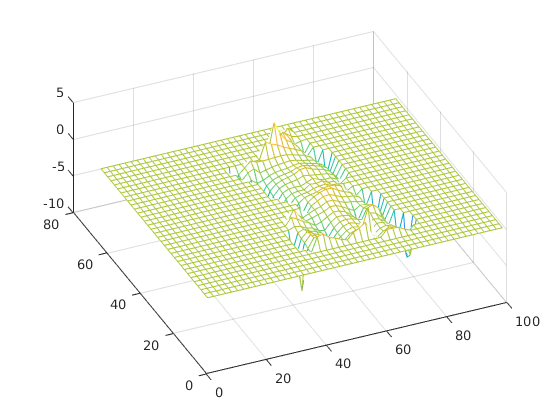
\includegraphics[width=.4\linewidth]{imagenes/gato_small_model_123.png}
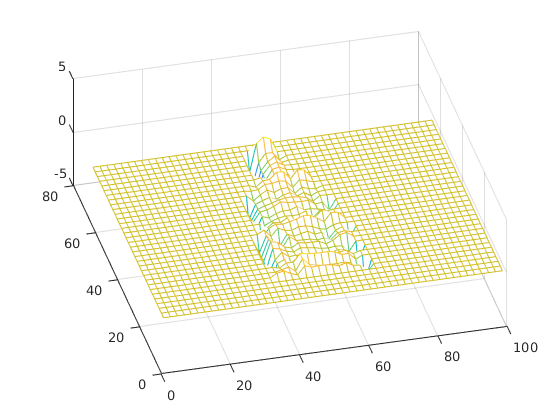
\includegraphics[width=.4\linewidth]{imagenes/buda_small_model_123.png}
\end{center}

\begin{center}
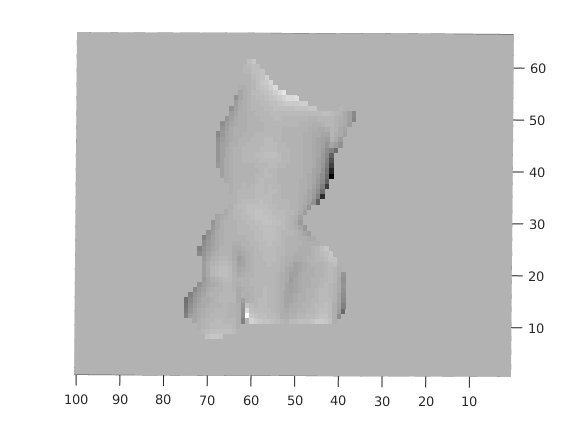
\includegraphics[width=.4\linewidth]{imagenes/gato_small_dephs_123.png}
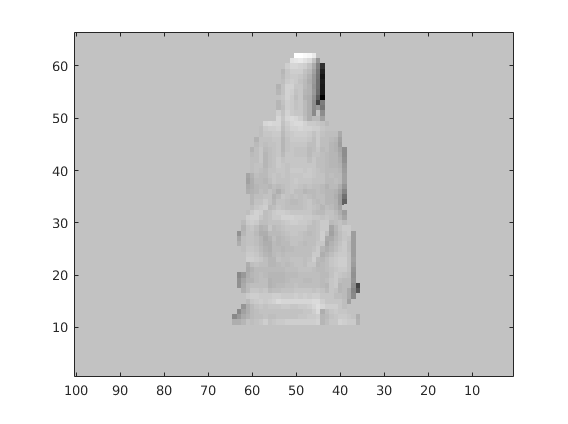
\includegraphics[width=.4\linewidth]{imagenes/buda_small_dephs_123.png}
\end{center}

En esta primera comparación se notó que el modelo y las profundidades del gato tenían una forma mejor detallada que el buda, aunque sólo con esta primera idea no se obtuvo ninguna conclusión, por lo que se continuó con las luces 4, 5 y 6. Sin embargo, al querer utilizar ese conjunto de luces se obtuvieron resultados completamente vacíos. La conclusión a la que se llegó para poder explicar este suceso luego de realizar pruebas fijando una y después dos luces, y cambiando las otras, fue que las luces 3 y 5 son vectores que no son linealmente independientes, ya que dejando fijas esas luces siempre se obtenían modelos vacíos. La razón por la que se concluyó que las luces 3 y 5 no son $L.I.$ fue que al hacer eliminación gausseana, se obtenían filas de $0$s y eso es lo que luego generaría $0$s en las normales estimadas y por lo tanto en todo el modelo.

Después de ese pequeño análisis, se precedió a realizar la generación de modelos 3D con las luces 7, 8 y 9 y los modelos obtenidos fueron los siguientes:

\begin{center}
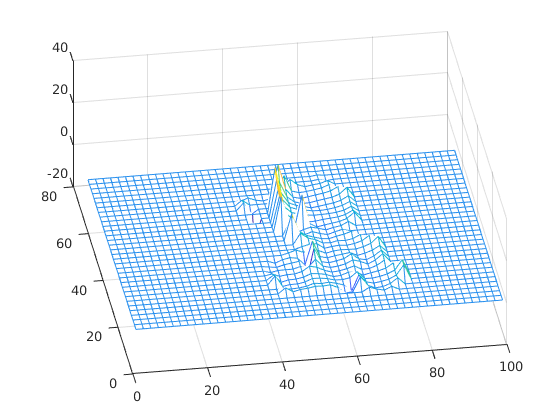
\includegraphics[width=.4\linewidth]{imagenes/gato_small_model_789.png}
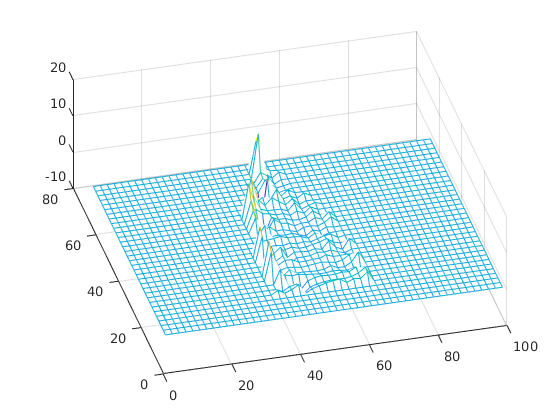
\includegraphics[width=.4\linewidth]{imagenes/buda_small_model_789.png}
\end{center}

\begin{center}
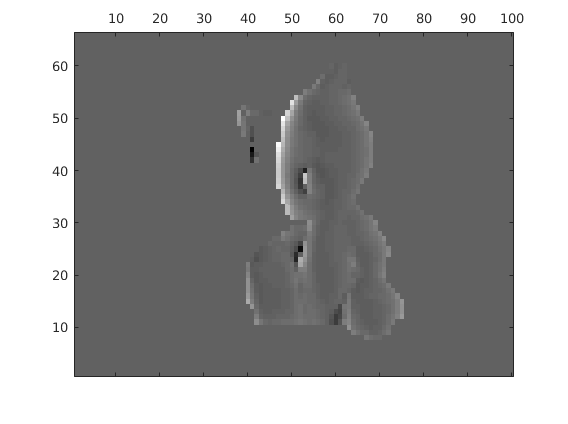
\includegraphics[width=.4\linewidth]{imagenes/gato_small_dephs_789.png}
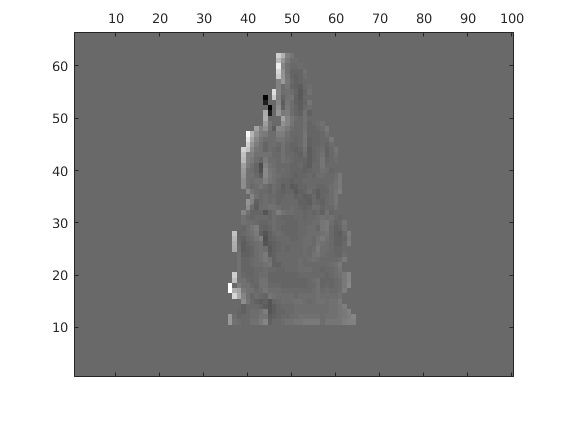
\includegraphics[width=.4\linewidth]{imagenes/buda_small_dephs_789.png}
\end{center}

Tras generar este segundo conjunto de imágenes se notó que ambos modelos tenían fallas muy marcadas ambos en la parte superior izquierda. Por lo tanto, se decidió reconstruir el modelo del mate para poder hacer una comparación más y el resultado obtenido fue el siguiente:

\begin{center}
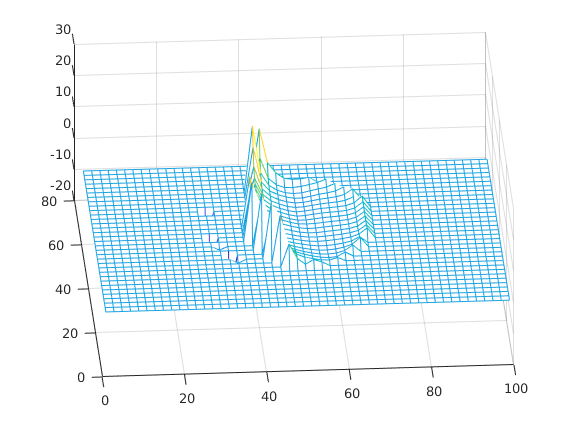
\includegraphics[width=.4\linewidth]{imagenes/mate_small_model_789.png}
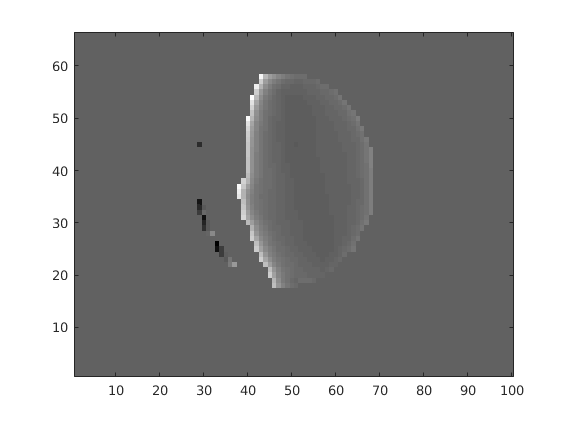
\includegraphics[width=.4\linewidth]{imagenes/mate_small_dephs_789.png}
\end{center}

Esta reconstrucción permitió concluir que las luces que se utilizaron provenían todas del lado derecho, generando una sombra en la parte izquierda de los objetos y eso permitió explicar por qué en las tres figuras habían partes faltantes en ese lado.

También se probó a utilizar las luces 10, 11 y 12, pero se obtuvo exactamente el mismo resultado que con 4, 5 y 6, por lo que se concluyó lo mismo que para estas últimas, solo que para las luces 10 y 12.

Por último, se probó a utilizar las luces 1, 5 y 11 ya que se observó que para algunos modelos andaba bastante mejor que las combinaciones probadas con anterioridad. Los resultados para el gato, el buda y el mate fueron los siguientes:

\begin{center}
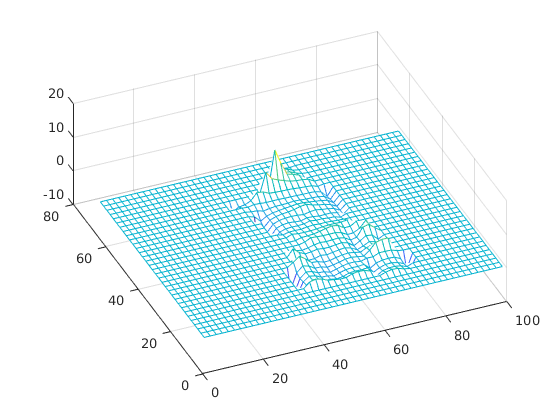
\includegraphics[width=.4\linewidth]{imagenes/gato_small_model_1511.png}
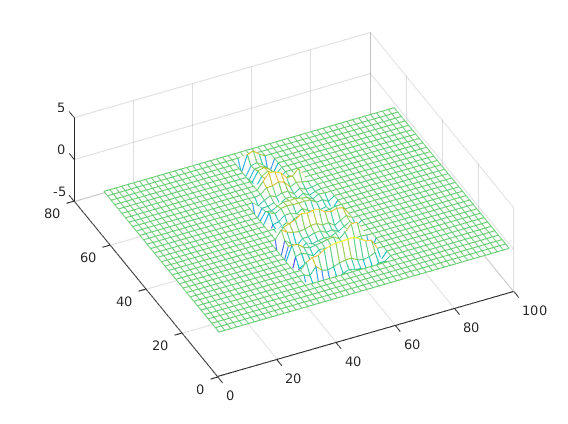
\includegraphics[width=.4\linewidth]{imagenes/buda_small_model_1511.png}
\end{center}

\begin{center}
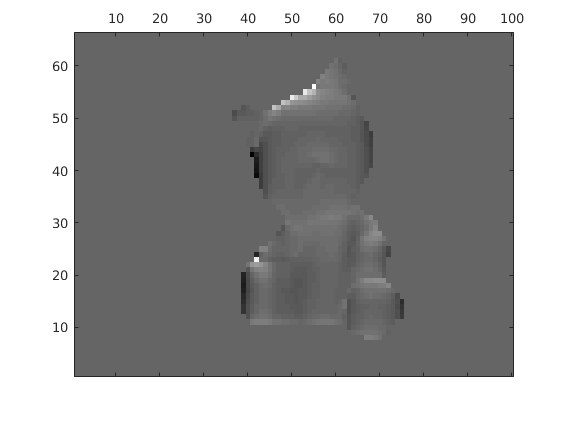
\includegraphics[width=.4\linewidth]{imagenes/gato_small_dephs_1511.png}
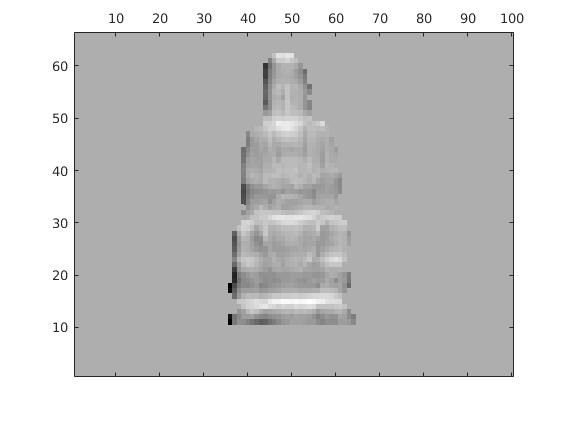
\includegraphics[width=.4\linewidth]{imagenes/buda_small_dephs_1511.png}
\end{center}

\begin{center}
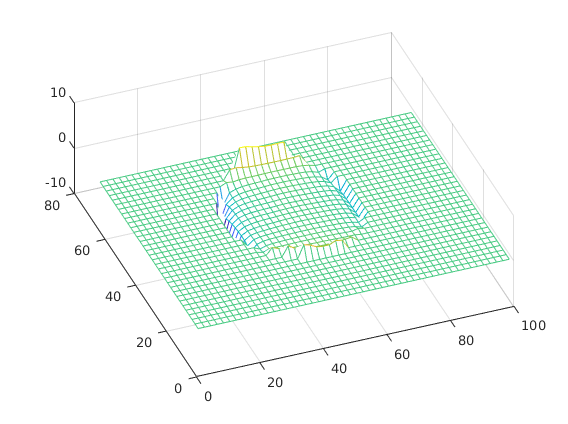
\includegraphics[width=.4\linewidth]{imagenes/mate_small_model_1511.png}
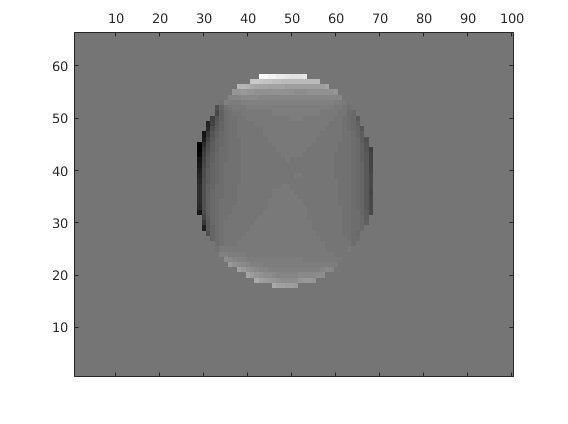
\includegraphics[width=.4\linewidth]{imagenes/mate_small_dephs_1511.png}
\end{center}

Se observó entonces con estos resultados que las luces elegidas efectivamente dieron un resultado diferente a los anteriores y además, con una calidad superior, ya que los tres modelos se asemejan bastante a los objetos reales a pesar de tener ciertas deformaciones como se ve en el caso del buda.
